\chapter{Systèmes de numérotation}
\section{Représentation des nombres}
Soit un nombre $N$ en base $r$, sa forme généralisé s'écrit:
\begin{equation}
	N = \underbrace{\sum_{i=0}^{i=n}a_ir^i}_{\text{Partie entière}} + \underbrace{\sum_{j=1}^{i=m}b_jr^{-j}}_{\text{Partie fractionnaire}}
\end{equation}
Les indexes $i,j$ s'appellent les poids. On distingue 2 parties:
\begin{itemize}
	\item Partie entière:  $n+1$ chiffres ($a_0,\dots,a_n$)
  \begin{itemize}
		\item $i=n$: bit de poids plus fort (Most Significant Bit (MSB))
	  \item $i=0$: bit de poids le plus faible (Least Significant Bit (LSB), donné par $\frac{N-a_0}{r}$)
	  \end{itemize}
	\item Partie fractionnaire: $m$ chiffres ($b_1,\dots,b_m$)
\end{itemize}
Parmi l'infinité de bases $r$ possibles, on en distingue 4:
\begin{table}
	\centering
	\begin{tabular}{|c|c|}
		\hline
		Type         & Base                                \\
		\hline
		Décimale    & \{0,1,2,3,4,5,6,7,8,9\}             \\
		Binaire      & \{0,1\}                             \\
		Octal        & \{0,1,2,3,4,5,6,7\}                 \\
		Hexadécimal & \{0,1,2,3,4,5,6,7,8,9,A,B,C,D,E,F\} \\
		\hline
	\end{tabular}
	\caption{Bases utiles}
	\label{bases utiles}
\end{table}
\section{Conversions}
De manière générale, pour passer d'une base $p$ à une base $q$, on fera $(N)_p\rightarrow (N)_{10}\rightarrow (N)_q$. \\

Pour passer de la base $p$ à la base $10$, il suffit de réécrire le nombre sous sa forme générale et de calculer le résultat. \\
Pour passer de la base $10$ à la base $q$, il faut séparer la partie entière de la fractionnaire :
\begin{itemize}
	\item Partie entière : diviser par la base $q$, noter le reste de la division et répéter l'opération jusqu'à ce que le nombre soit plus petit que $q$. Une fois le résultat obtenu, le chiffre résultant se lit dans le sens \textbf{contraire} que celui du calcul. Exemple :
	\begin{figure}[H]
		\centering
		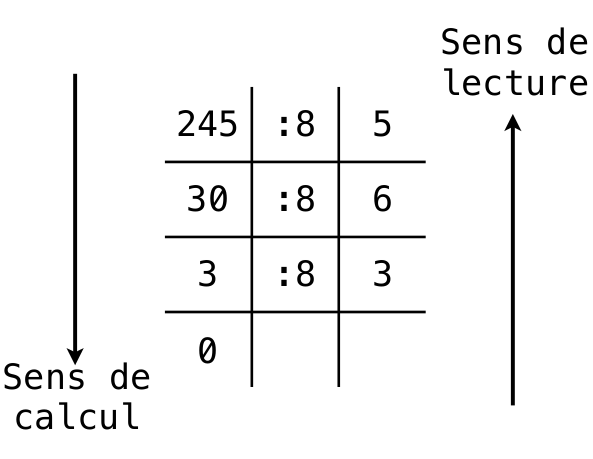
\includegraphics[scale=0.25]{ch1/image1}
	\end{figure}
	\item Partie fractionnaire : écrire la partie fractionnaire sous la forme $0.xxx...$, la multiplier par $q$, noter la partie entière, réinitialiser la partie entière à $0$ et répéter l'opération. Le nombre résultant se lit dans le \textbf{même} sens que celui du calcul. Exemple :
	\begin{figure}[H]
		\centering
		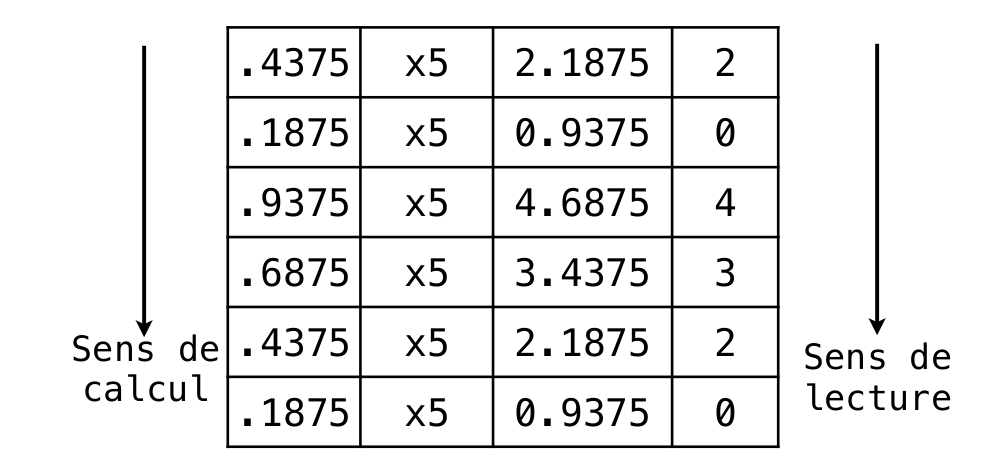
\includegraphics[scale=0.22]{ch1/image2}
	\end{figure}
\end{itemize}
\danger Faire gaffe avec l'hexadécimal, ne pas oublier de remplacer les chiffres $>9$ par les lettres correspondantes\\

Néanmoins, dans le cas des bases utiles (\autoref{bases utiles}), on préférera passer par la base 2. En effet, il suffit de regrouper les chiffres par groupe de $x$ ($2^x=$ nouvelle base), exemple: $x=4$ pour la base $2\leftrightarrow 16$). On regroupera les chiffres en partant de part et d'autre de la virgule.
\begin{figure}[H]
	\centering
	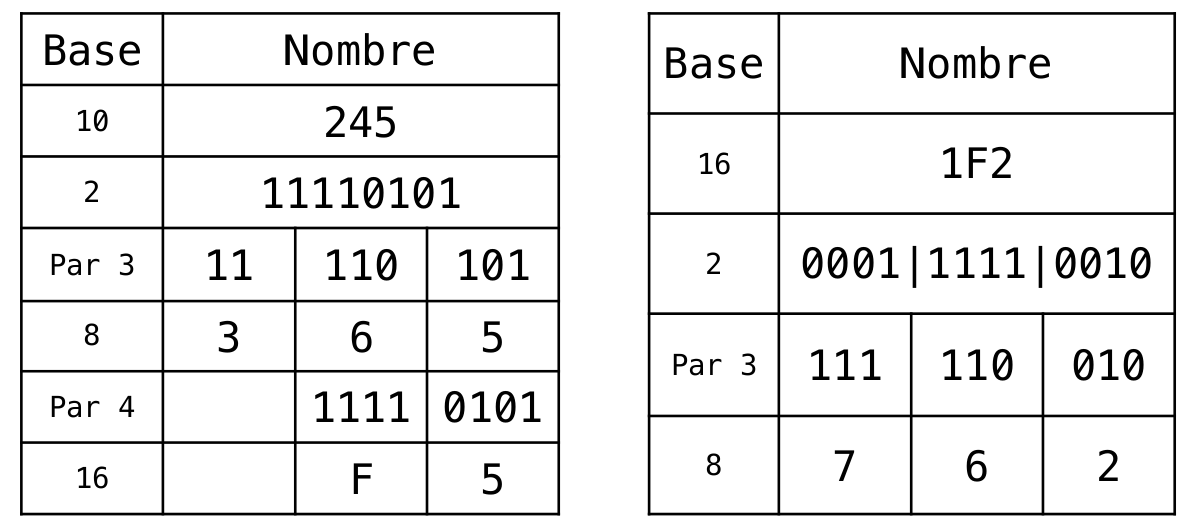
\includegraphics[scale=0.2]{ch1/image3}
	\caption{Conversion entre bases utiles}
\end{figure}
\danger Surtout ne pas oublier les chiffres manquants pour la partie fractionnaire
\paragraph{Astuce} En binaire, lorsqu'un nombre est composé majoritairement de 1 et qu'on veut sa valeur, comme le nombre $111110010$, comptez le nombre de chiffre $\Rightarrow x$, faire $2^x-1$ et soustraire $2^i$ ($i=$ poids de chaque 0). Dans notre exemple :
\begin{align}
	(111110010)_2 &=(?)_{10}\\
	x &=9\\
	2^9-1 &=(511)_{10}\\
	511-2^0-2^2-2^3 &=(498)_{10}\\
	(111110010)_2 &=(498)_{10}
\end{align}
\section{Opération arithmétiques}
Les additions, soustractions, multiplications et divisions se déroulent comme en base 10, si ce n'est qu'au lieu de reporter quand on arrive au-dessus de 9, on reporte quand on arrive au dessus de la base$-1$ (grosso modo). Voir TP 1
\paragraph{Remarque} dans le cas de codage binaire sur 8 bits (chiffre maximum 255), si l'on fait $236+170$, nous obtenons un chiffre au-dessus de la limite pour 8 bits, nous aurons donc un 9\up{ème} bit. Le résultat sera donc tronqué car codé sur 8 bits.Ce problème de débordement s'appelle l'\textit{overflow}
\section{Nombres négatifs}
En binaire, il existe 3 modes de représentation pour les nombres négatifs :
\begin{enumerate}
	\item Signe et Valeur Absolue (SVA)
	\item Complément à la base ($C_1$)
	\item Complément à 2 ($C_2$)
\end{enumerate}
\subsection{Signe et Valeur Absolue (SVA)}
\label{subsec:sva}
Par convention :
\begin{itemize}
	\item 1 bit réservé pour le signe tel que :
	\begin{itemize}
		\item $0 =$ positif
		\item $1=$ négatif
	\end{itemize}
	\item le reste réservé pour la valeur absolue
\end{itemize}
Ainsi, sur un mode à 8 bits, on peut représenter des chiffres $\in [-127,127]$\\
Pour faire des opérations arithmétiques avec cette notation, il faut :
\begin{enumerate}
	\item Comparer les signes pour déterminer le signe des résultats
	\item Comparer la magnitude des nombres pour déterminer le sens ($A<B\rightarrow B-A$,\\ $A>B\rightarrow A-B$)
\end{enumerate}
Niveau matériel, c'est galère\dots
\subsection{Complément à la base}
\subsubsection{Complément à 1 ($C_1$)}
Cette notation est valable $\forall$ base. Le principe est de faire la soustraction comme une addition.\\
Soit 2 nombre $A$ et $B$, en base $r$, codés sur $m$ chiffres
\begin{align}
	A-B &= A + (-B) & \\
	&= A + (r^m-B) = A+B'  &  \text{où}
	\begin{array}{l}
		B' = \text{complément à la base }r\\
		B+B'=r^m
	\end{array}
\end{align}

Mais pour arriver à ça, il faut quand même faire la soustraction $r^m-B$. Réorganisons
\begin{equation}
	B'=(r^m-B)=((r^m-1)-B)+1
\end{equation}
$(r^m-1)-B$ est un complément de chaque chiffre de $B$
\begin{align}
	(r^m-1)-B &=(\underbrace{(r-1)\ (r-1)}_{\text{\danger Concaténation}}\dots\ (r-1)-(b_{m-1}\ b_{m-2}\dots\ b_0)\\
	&= ((r-1)-b_{m-1}((r-1)b_{m-2})\dots((r-1)-b_0)\\
	&= b'_{m-1}\ b'_{m-2}\dots\ b'_0
\end{align}
Cette méthode est très pratique en \textbf{binaire}, chaque chiffre est simplement inversé! Seul problème, nous avons 2 manière de représenter le 0 (sur 8 bits: $0000000$ et $11111111$). Les opérations arithmétique en $C_1$ sont faisable mais comporte parfois quelques cas particuliers.
\subsubsection{Complément à 2 ($C_2$)}
Au lieu d'utiliser le complément à 1 : $B'=(r^m-1)-B$, on utilise le complément à 2 : $B'=(r^m-1)-B+1$. Grosso modo, on ajoute 1 au complément à 1. Contrairement à $C_1$ et SAV, on peut représenter les nombre $\in [-128,127]$ et nous n'avons qu'une notation pour 0. La conséquence de tout ça est qu'il sera beaucoup plus facile de faire des opération arithmétique (soustraction $\Rightarrow$ sommation). Seul problème, l'overflow\dots
\subsubsection{Méthode de conversion pour complément}
Nous utiliserons la plupart du temps le complément à 2. Pour convertir un nombre en complément à 1 ou 2 rien de plus simple: 
\begin{enumerate}
	\item Prendre la valeur absolue du nombre en \textbf{base 2} et compléter avec des 0 pour avoir les $m$ bits demandés
	\item Si le nombre est négatif: 
	\begin{enumerate}
		\item Inverser chaque bit $\Rightarrow C_1$
		\item $C_1+1\Rightarrow C_2$
	\end{enumerate}
\end{enumerate}
\subsection{Overflow en $C_2$}
une règle très simple permet de savoir si nous somme en overflow ou si le bit débordant peut être oublié sans risque
\begin{center}
	Si les 2 derniers bits du résultats sont \textbf{différent} (01 ou 10)$\Rightarrow$ \textbf{OK}\\
	Si les 2 derniers bits du résultats sont \textbf{les mêmes} (11 ou 00) $\Rightarrow$ \textbf{Overflow}
\end{center}
\section{Virgule flottante : Forme généralisée}
Les nombres en virgule fixe à 32 ou 64 bits limitent fortement les calculs et augmenter le nombre de bit n'est pas une solution $\rightarrow$ Nombre en virgule flottante:
\begin{equation}
N=mantisse\times(base)^{exposant}
\end{equation}
\subsection{Standard IEEE 754}
On distingue 2 types de précision:
\begin{itemize}
	\item Simple précision: 32 bits\\
	\begin{table}[H]
		\centering
		\begin{tabular}{|c|c|c|c|}
			\hline
			Nombre de bits & 1 & 8 & 23\\
			\hline
			Type & Signe de la mantisse & Exposant (0 à 255) & Fraction normalisée\\
			\hline
			Biais & & 127 &\\
			\hline
		\end{tabular}
		\caption{IEEE 754 - Simple Précision}
	\end{table}
	\item Double précision: 64 bits\\
	\begin{table}[H]
		\centering
		\begin{tabular}{|c|c|c|c|}
			\hline
			Nombre de bits & 1 & 11 & 52\\
			\hline
			Type & Signe de la mantisse & Exposant (0 à 2047) & Fraction normalisée\\
			\hline
			Biais & & 1023 &\\
			\hline
		\end{tabular}
		\caption{IEEE 754 - Double Précision}
	\end{table}
\end{itemize}
Pour convertir un chiffre en virgule flottante il faut:
\begin{enumerate}
	\item Convertir le nombre en binaire
	\item Mettre sous forme $1.abcd...\ (\times x)$
	\item Déterminer le signe (0 ou 1, voir \autoref{subsec:sva})
	\item Calculer l'exposant: $E=x+biais$
	\item Écrire la mantisse ($abcd...$) 
\end{enumerate}
\danger Le 1 de $1.abcd...$ n'est pas a écrire dans la mantisse